\documentclass{article}
\usepackage{tikz}

\begin{document}
\thispagestyle{empty}
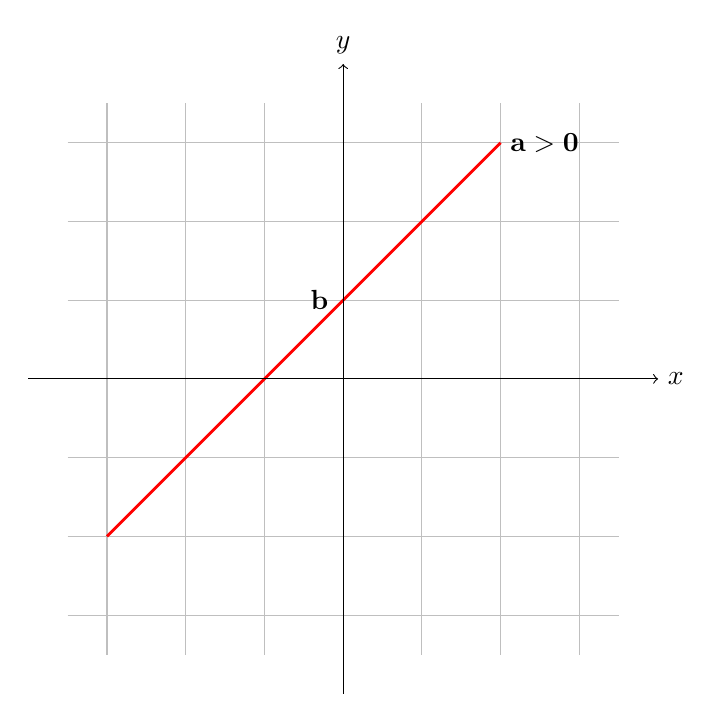
\begin{tikzpicture}[scale=1]
% Desenhar o grid com coordenadas x e y
\draw[step=1,gray!50] (-3.5,-3.5) grid (3.5,3.5);
% Desenhar a reta diagonal com espessura thick e ângulo de 45 graus
\draw[line width=1pt, red] (-3,-2) -- (2,3);
% Colocar um nó com a letra "b" no ponto (0,2)
\node at (-0.3,1) {$\bf b$};
\node[right] at (2,3) { $\bf a > 0$};
% Etiquetas dos eixos x e y
\draw[->] (-4,0) -- (4,0) node[right] {$x$};
\draw[->] (0,-4) -- (0,4) node[above] {$y$};
\end{tikzpicture}
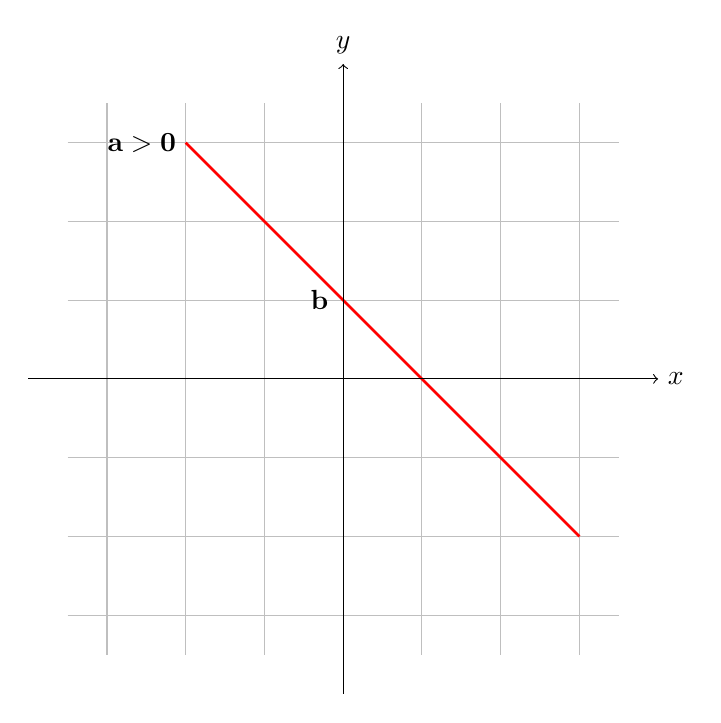
\begin{tikzpicture}[scale=1]
% Desenhar o grid com coordenadas x e y
\draw[step=1,gray!50] (-3.5,-3.5) grid (3.5,3.5);
% Desenhar a reta diagonal com espessura thick e ângulo de 45 graus
\draw[line width=1pt, red] (3,-2) -- (-2,3);
% Colocar um nó com a letra "b" no ponto (0,2)
\node at (-0.3,1) {$\bf b$};
\node[left] at (-2,3) { $\bf a > 0$};
% Etiquetas dos eixos x e y
\draw[->] (-4,0) -- (4,0) node[right] {$x$};
\draw[->] (0,-4) -- (0,4) node[above] {$y$};
\end{tikzpicture}

\end{document}
